\section{Robustness, Placebo and Power}\label{sec:robustness}

\paragraph*{Pre-registered checks} Table~\ref{tab:robust} and Fig.~\ref{fig:robust} report the closed list of ten robustness checks next to the baseline: a break at Senate passage; a placebo break; dropping $\pm$10 business days around the Terra, FTX and SVB episodes; USDT-only and USDC-only flows; the all-USD-pegged aggregate; the one-day timing shift; flow windows of one and ten days; and lags-only controls. Across the \rbN{} non-placebo rows $\delta_{10}$ is never significant (smallest \rbMinP{}) and is positive in \rbNPos{} of them. The exception is USDT-only flows, where the post-enactment response is larger (\rbUSDTPost{} against \rbUSDTPre{}\,bp; $\delta_{10}=\rbUSDTDiff{}$, \rbUSDTDiffP{}). The post-enactment response is individually significant only with the all-USD-pegged aggregate (\rbAllPost{}\,bp, \rbAllPostP{}) and the ten-day window (\rbKtenPost{}\,bp, \rbKtenPostP{}).

\paragraph*{Placebo} A break on 18~July 2024, estimated on data ending before Senate passage, gives $\delta_{10}=\rbPlDiff{}$\,bp (\rbPlDiffP{}), with a ``post'' response of \rbPlPost{}\,bp. The flow--yield association thus shifts by more than the GENIUS-Act difference between two sub-periods separated by no legislative event. Even a significant $\delta_{10}$ at enactment could not have been attributed to the Act on this evidence, and the instability is itself a finding: the controls-only association is not a stable structural parameter.

\paragraph*{Power} With \nPostTen{} post-enactment observations at $h=10$, the standard error of $\delta_{10}$ is \bDiffSE{}\,bp. The minimum detectable difference at 80\% power and a two-sided 5\% test is therefore about $2.8\times\bDiffSE{}\approx\mde{}$\,bp per USD~10\,bn, roughly \mdeRatio{} times the entire pre-enactment estimate. A doubling of the response would have been hard to detect. The null is weak evidence of no change.

\begin{figure}[!t]
\centering
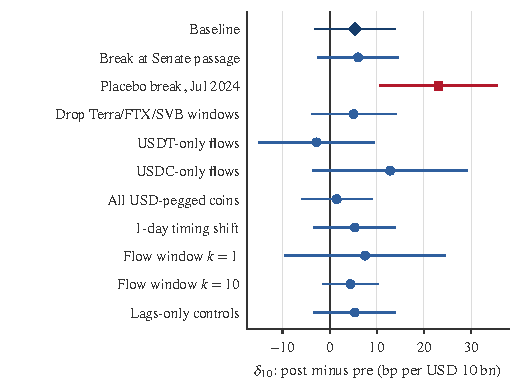
\includegraphics[width=\columnwidth]{figures/fig_robust.pdf}
\caption{Pre-registered robustness: the change at enactment $\delta_{10}$ (post minus pre, bp per USD~10\,bn of $k$-day flow) with 90\% Newey--West intervals. Diamond: baseline. Square: placebo break on 18~July 2024, estimated on data ending 16~June 2025.}
\label{fig:robust}
\end{figure}

\begin{table*}[!t]
\centering
\caption{Robustness (pre-registered): 3-month bill, $h=10$, estimate (s.e.)}
\label{tab:robust}
\footnotesize
\begin{adjustbox}{max width=\textwidth}
% generated by src/viz/paper_tex.py
\begin{tabular}{lrrrrr}
\toprule
Specification ($h=10$, per USD 10\,bn) & Pre $\beta$ & Post $\beta+\delta$ & $\delta$ & $p(\delta)$ & $N_{pre}$\,/\,$N_{post}$ \\
\midrule
Baseline (primary spec) & \ensuremath{-}10.90 (4.16) & \ensuremath{-}5.56 (4.54) & +5.35 (5.21) & 0.30 & 1135\,/\,312 \\
Alternative break 2025-06-17 (Senate) & \ensuremath{-}10.89 (4.19) & \ensuremath{-}4.86 (4.50) & +6.03 (5.18) & 0.24 & 1114\,/\,333 \\
\midrule
Placebo break 2024-07-18 (data to 2025-06-16) & \ensuremath{-}13.46 (4.76) & 9.64 (6.60) & +23.10 (7.58) & $<$0.01 & 886\,/\,218 \\
\midrule
Drop $\pm$10 business days around Terra, FTX, SVB & \ensuremath{-}10.67 (4.51) & \ensuremath{-}5.55 (4.57) & +5.12 (5.50) & 0.35 & 1072\,/\,312 \\
USDT-only flows & \ensuremath{-}10.67 (4.87) & \ensuremath{-}13.45 (7.08) & \ensuremath{-}2.79 (7.46) & 0.71 & 1135\,/\,312 \\
USDC-only flows & \ensuremath{-}16.58 (9.55) & \ensuremath{-}3.75 (8.52) & +12.83 (9.98) & 0.20 & 1135\,/\,312 \\
All USD-pegged aggregate & \ensuremath{-}10.74 (2.62) & \ensuremath{-}9.23 (4.42) & +1.51 (4.60) & 0.74 & 1135\,/\,312 \\
1-day timing shift & \ensuremath{-}11.06 (4.41) & \ensuremath{-}5.72 (4.31) & +5.34 (5.30) & 0.31 & 1135\,/\,312 \\
Flow window k = 1 & \ensuremath{-}11.54 (4.84) & \ensuremath{-}4.02 (7.98) & +7.51 (10.33) & 0.47 & 1135\,/\,312 \\
Flow window k = 10 & \ensuremath{-}12.42 (3.98) & \ensuremath{-}8.01 (2.69) & +4.42 (3.63) & 0.22 & 1135\,/\,312 \\
Lags-only controls & \ensuremath{-}11.01 (4.41) & \ensuremath{-}5.65 (4.54) & +5.35 (5.28) & 0.31 & 1135\,/\,312 \\
\bottomrule
\end{tabular}

\end{adjustbox}

\vspace{2pt}
\parbox{\textwidth}{\footnotesize ``Pre'' and ``post'' are relative to each row's break date; in the placebo row ``post'' is 18~July 2024 to 16~June 2025 and the GENIUS period is outside the sample. USDT- and USDC-only rows use that coin's own flows; the $k$ rows change the flow window, so ``per USD 10\,bn'' refers to a $k$-day flow.}
\end{table*}
